\documentclass{memoir}
\usepackage{lipsum}
\usepackage[pass]{geometry}
\usepackage[utf8]{inputenc}
\usepackage{amsmath}
\usepackage{amssymb}
\usepackage[T1]{fontenc}
\usepackage[shortlabels]{enumitem}
\usepackage[polish]{babel}
\usepackage[table,xcdraw]{xcolor}
\newdimen\lastlinewidth
\usepackage{graphicx}
\usepackage{subfig}
\usepackage{listings}
\usepackage{subfig}
\usepackage{enumitem}
\graphicspath{ {./} }
\usepackage{parskip}
\usepackage{multirow}
\usepackage{placeins}
\title{Lista 1}
\author{Mateusz Biłyk}

\begin{document}
\maketitle
\section*{Zadanie 1}
Wygeneruj n obserwacji z rozkładu $\mathcal{N}(\theta,\sigma^2$). Na tej podstawie oblicz wartość estymatora parametru $\theta$ postaci:
\begin{enumerate}
	\item $\hat{\theta_1}=(1/n)\sum X_i$
	\item $\hat{\theta_2}=Me\{X_1,...,X_n\}$
	\item $\hat{\theta_3}=X_1$
	\item $\hat{\theta_4}=\sum w_i X_{i:n}$, gdzie $X_{1:n}\leq ... \leq X_{n:n}$ 
są uporządkowanymi obserwacjami  
	$X_1,...,X_n$, $$w_i= \varphi \left( \Phi^{-1} \left( \frac{i-1}{n} \right) \right) - \varphi \left( \Phi^{-1} \left( \frac{i}{n} \right) \right)$$
	przy czym $\varphi$ jest gęstością, a $\Phi$ dystrybuantą standardowego rozkładu normalnego $\mathcal{N}(0,1)$.
	Doświadczenie powtórz 10000 razy. Na tej podstawie oszacuj wariancję, błąd średniokwadratowy oraz obciążenie każdego z estymatorów. Przedyskutuj otrzymane wyniki.
\end{enumerate}

\begin{enumerate}[a)]
\item $n=50$,$\theta=1$,$\sigma=1$
\begin{table}[htb]
\centering
\begin{tabular}{|
>{\columncolor[HTML]{DAE8FC}}l |lll}
\hline
 & \multicolumn{1}{l|}{\cellcolor[HTML]{DAE8FC}Var} & \multicolumn{1}{l|}{\cellcolor[HTML]{DAE8FC}MSE} & \multicolumn{1}{l|}{\cellcolor[HTML]{DAE8FC}b} \\ \hline
$\hat{\theta}_1$ & 0.02 & 0.02 & 0.001   \\ \cline{1-1}
$\hat{\theta}_2$ & 0.03 & 0.03 & 0.0009  \\ \cline{1-1}
$\hat{\theta}_3$ & 1    & 1    & -0.0006 \\ \cline{1-1}
$\hat{\theta}_4$ & 0.01 & 0.01 & -0.03   \\ \cline{1-1}
\end{tabular}
\end{table}
\newpage
\item $n=50$,$\theta=4$,$\sigma=1$
\begin{table}[htb]
\centering
\begin{tabular}{|
>{\columncolor[HTML]{DAE8FC}}l |lll}
\hline
 & \multicolumn{1}{l|}{\cellcolor[HTML]{DAE8FC}Var} & \multicolumn{1}{l|}{\cellcolor[HTML]{DAE8FC}MSE} & \multicolumn{1}{l|}{\cellcolor[HTML]{DAE8FC}b} \\ \hline
$\hat{\theta}_1$ & 0.02 & 0.02 & 0.001 \\ \cline{1-1}
$\hat{\theta}_2$ & 0.03 & 0.03 & 0.001 \\ \cline{1-1}
$\hat{\theta}_3$ & 1    & 1    & 0.01  \\ \cline{1-1}
$\hat{\theta}_4$ & 0.01 & 9    & -3    \\ \cline{1-1}
\end{tabular}
\end{table}
\item $n=50$,$\theta=1$,$\sigma=2$
\begin{table}[htb]
\centering
\begin{tabular}{|
>{\columncolor[HTML]{DAE8FC}}l |lll}
\hline
 & \multicolumn{1}{l|}{\cellcolor[HTML]{DAE8FC}Var} & \multicolumn{1}{l|}{\cellcolor[HTML]{DAE8FC}MSE} & \multicolumn{1}{l|}{\cellcolor[HTML]{DAE8FC}b} \\ \hline
$\hat{\theta}_1$ & 0.08 & 0.08 & -0.002 \\ \cline{1-1}
$\hat{\theta}_2$ & 0.12 & 0.12 & -0.003 \\ \cline{1-1}
$\hat{\theta}_3$ & 4    & 4    & 0.002  \\ \cline{1-1}
$\hat{\theta}_4$ & 0.04 & 1    & 1      \\ \cline{1-1}
\end{tabular}
\end{table}
\end{enumerate}
\textit{Jak można było łatwo przewidzieć, czwarty estymator radzi sobie najlepiej w przypadku a) w innych  przypadkach jest tragiczny bo po prostu nie jest do tego stworzony. Zawsze porządnie działa naturalny estymator jakim jest średnia, co też nie jest żadną niespodzianką. Wybrałem taki estymator numer 3, aby mieć możliwość porównania naszych wyników z wynikami bardzo głupiego estymatora zwracającego zawsze pierwszy element. Można zauważyć, że taki estymator obciążenie ma często bardzo małe. Ciekawą obserwacją jest, że w podpunkcie c) wariancja wszystkich estymatorów zwiększyła się zgodnie dokładnie 4 razy. Oczywiście wynika to ze zwiększenia przez nas wartości $\sigma$.}
\section*{Zadanie 2}
Omów komendę set.seed(1) oraz jej potencjalne zastosowania.
\textit{Jest to komenda, która ustala ziarno losowości w naszym programie. Na jego podstawie nasz algorytm będzie pseudo losował liczby. Jeżeli  ustawimy to samo ziarno losowości program wylosuje nam za każdym razem te same liczby, więc aby zwiększać losowość naszego programu możemy za ziarno losowości obrać czas systemowy lub adres następnej wolnej komórki w pamięci. Te wartości się bardzo szybko zmieniają, więc tak skonstruowane ziarno losowości może dać lepsze rezultaty.}
\section*{Zadanie 3}
Omów konieczność numerycznego wyznaczania estymatorów największej wiarygodności na przykładzie estymacji parametru przesunięcia w rozkładzie logistycznym.\textit{Czasami, tak jak w przykładzie estymacji parametru przesunięcia w rozkładzie logistycznym, jesteśmy w stanie udowodnić, że istnieje unikalny estymator, ale nie jesteśmy w stanie podać prostego wzoru, który by go wyliczał. W takiej sytuacji można zastosować na przykład prosty algorytm Newtona i bez problemów oszacować nasz estymator. }
\section*{Zadanie 4}
Omów wybraną metodę numeryczną pozwalającą na wyznaczanie estymatora największej wiarygodności. \textit{Wspominana we wcześniejszym zadaniu metoda Newtona jest metodą numeryczną, która w jest w stanie numerycznie przybliżać nam estymator największej wiarygodności. Takim estymatorem może być Maximum Likelihood Estimator, którego zadaniem jest szacowanie parametru w taki sposób, aby zdarzenie otrzymania naszych danych miało maksymalne prawdopodobieństwo. Po rozpisaniu równań bardzo często nasz problem upraszcza się do znalezienia zera jakiejś funkcji i w tym metoda Newtona może być nam pomocna. Polega ona na tym, że na początku zgadujemy miejsce zerowe $x_0$, a potem używając wzoru na styczną do naszej funkcji $x_{n+1}=x_n - f(x_n)/f'(x_n)$ tworzymy kolejne przybliżenia miejsca zerowego, aż dokładność będzie satysfakcjonująca. Moja implementacha metody Newtona:}
\begin{verbatim}
newtons_method <- function(f,df,x0,k,alp){
  x<-x0
  for(i in 1:k){
    x <- x-alp*(f(x)/df(x))
  }
  if(is.na(x) || is.infinite(x)){
    return(NaN)
  }
  if(f(x) < 10^(-6)&&abs(x-x0)<0.5){
    return (x)
  }else {
      return(NaN)
  }
}
\end{verbatim}
\textit{Parametry w mojej funkcji to po kolei: badana funkcja, jej pochodna,punkt startowy,ilość kroków, szybkość zmian. Wprowadzam parametr alp, który jest odpowiedzialny za prędkość zmian w naszym programie. Zwykle ustawiałem go na 0.1. Jest on potrzebny gdyż bez niego często nasz program potrafi wystrzeliwać do nieskończoności. Procedura jest standardowa, następnie pierwszy if sprawdza czy wyszła nam w ogóle liczba a drugi czy ma ona jakiś sens, czyli czy jest to przybliżenie zera funkcji f oraz czy nie wyszliśmy za daleko poza przedział, w którym wiemy że funkcja f się zeruje. }
\section*{Zadanie 5}
Wygeneruj $n$ obserwacji z rozkładu logistycznego $\mathcal{L}(\theta,\sigma)$ z parametriem przesunięcia $\theta$ i skali $\sigma$. Oszacuj wartość estymatora największej wiarygodności parametru $\theta$ na podstawie wygenerowanej próby. Przedyskutuj wybór punktu początkowego oraz liczbę kroków w algorytmie. Doświadczenie powtórz 10000 razy. Na tej podstawie oszacuj wariancję, błąd średniokwadratowy oraz obciążenie estymatora. Przedyskutuj uzyskane wyniki.
\textit{Za punkt początkowy obierałem losowe punkty aż dostałem rozsądne wyniki (nie będące NaN-em), gdyż jest na najpraktyczniejsza metoda. Liczbę kroków w algorytmie Newtona ustawiłem na 1000, bo jest to wystarczająca ilość, aby w krótkim czasie dostać bardzo dobre przybliżenia punktów zerowej naszej funkcji:} $$l'(\theta)=-\sum \frac{\tanh \left( \frac{\theta-x_i}{2\sigma} \right)}{\sigma} $$
\begin{enumerate}[a)]
\item $n=50$,$\theta=1$,$\sigma=1$\\
\textit{Wariancja:0.034, błąd średniokwadratowy:0.042, obciążenie: -0.088}
\item $n=50$,$\theta=4$,$\sigma=1$\\
\textit{Wariancja:0.04, błąd średniokwadratowy:0.07, obciążenie: -0.17}
\item $n=50$,$\theta=1$,$\sigma=2$\\
\textit{Wariancja:0.06, błąd średniokwadratowy:0.11, obciążenie: -0.21}
\end{enumerate}
\textit{Metoda Newtona sprawdza się bardzo dobrze do szacowania estymatora największej wiarygodności, pod warunkiem, że dostanie rozsądny punkt początkowy, a o to nie trudno. Wiadomo, że im większe ilość kroków w naszej metodzie tym lepsze przybliżenie, ale nie potrzeba ich wiele aby nasza procedura się już stabilizowała w jakimś punkcie. Zauważmy, że różnica pomiędzy wynikami w punkcie a) i b) polega na zmianie w obciążeniu, a różnica pomiędzy punktami b) i c) na różnicy w wariancji.  }
\section*{Zadanie 6}
Wygeneruj n obserwacji z rozkładu Cauch'ego $\mathcal{C}(\theta,\sigma)$ z parametrem przesunięcia $\theta$ i skali $\sigma$. Oszacuj wartość estymatora największej wiarygodności parametru $\theta$ na podstawie wygenerowanej próby. Przedyskutuj wybór punktu początkowego oraz liczbę kroków w algorytmie. Doświadczenie powtórz 10000 razy. Na tej podstawie oszacuj wariancję, błąd średniokwadratowy oraz obciążenie estymatora. Przedyskutuj uzyskane wyniki. \textit{Wszystkie parametry ustawiamy tak samo jak we wcześniejszym zadaniu tylko funkcje w metodzie Newtona zmieniamy, gdyż teraz chcemy zminimalizować funkcję:} $$ l'(\theta)= \sum \frac{2x_i - 2\theta}{(\theta-x_i)^2+\sigma^2}$$
\begin{enumerate}[a)]
\item $n=50$,$\theta=1$,$\sigma=1$\\
\textit{Wariancja:0.026, błąd średniokwadratowy:0.03, obciążenie: -0.06}
\item $n=50$,$\theta=4$,$\sigma=1$\\
\textit{Wariancja:0.02, błąd średniokwadratowy:0.03, obciążenie: -0.056}
\item $n=50$,$\theta=1$,$\sigma=2$\\
\textit{Wariancja:0.06, błąd średniokwadratowy:0.09, obciążenie: -0.176}
\end{enumerate}
\textit{ Podpunkty a) i b) się niczym nie różnią, dla naszego estymatora parametr $\theta$ nie ma znaczenia. Gdy zwiększamy wartość $\sigma$ w c) wariancja estymatora idzie w górę co pociąga powiększenie się błędu średniokwadratowego.}
\section*{Zadanie 7}
Powtórz eksperyment numeryczny z zadań 1,5 oraz 6 dla $n=20$ i $n=100$. Przedyskutuj uzyskane rezultaty w nawiązaniu do wcześniejszych wyników.
\begin{enumerate}[a)]
\item $n=20$,$\theta=1$,$\sigma=1$
\begin{table}[htb]
\centering
\begin{tabular}{|
>{\columncolor[HTML]{DAE8FC}}l |lll}
\hline
 & \multicolumn{1}{l|}{\cellcolor[HTML]{DAE8FC}Var} & \multicolumn{1}{l|}{\cellcolor[HTML]{DAE8FC}MSE} & \multicolumn{1}{l|}{\cellcolor[HTML]{DAE8FC}b} \\ \hline
$\hat{\theta}_1$ & 0.05 & 0.05 & -0.002   \\ \cline{1-1}
$\hat{\theta}_2$ & 0.07 & 0.07 & -0.003  \\ \cline{1-1}
$\hat{\theta}_3$ & 0.989 & 0.998  & 0.001 \\ \cline{1-1}
$\hat{\theta}_4$ & 0.023 & 0.028 & -0.067   \\ \cline{1-1}
\end{tabular}
\end{table}\\
\FloatBarrier
\textit{Rozkład Logistyczny: Wariancja:0.027, błąd średniokwadratowy:0.033, obciążenie: -0.08}\\
\textit{Rozkład Cauch'ego: Wariancja:0.026, błąd średniokwadratowy:0.03, obciążenie: -0.07}
\item $n=100$,$\theta=1$,$\sigma=1$
\begin{table}[htb]
\centering
\begin{tabular}{|
>{\columncolor[HTML]{DAE8FC}}l |lll}
\hline
 & \multicolumn{1}{l|}{\cellcolor[HTML]{DAE8FC}Var} & \multicolumn{1}{l|}{\cellcolor[HTML]{DAE8FC}MSE} & \multicolumn{1}{l|}{\cellcolor[HTML]{DAE8FC}b} \\ \hline
$\hat{\theta}_1$ & 0.01 & 0.01 & -0.002   \\ \cline{1-1}
$\hat{\theta}_2$ & 0.02 & 0.015 & -0.001  \\ \cline{1-1}
$\hat{\theta}_3$ & 1 & 1  & -0.02 \\ \cline{1-1}
$\hat{\theta}_4$ & 0.005 & 0.005 & -0.015   \\ \cline{1-1}
\end{tabular}
\end{table}\\
\FloatBarrier
\textit{Rozkład Logistyczny: Wariancja:0.018, błąd średniokwadratowy:0.0196, obciążenie: -0.0365}\\
\textit{Rozkład Cauch'ego: Wariancja:0.0145, błąd średniokwadratowy:0.0151, obciążenie: -0.025}
\item $n=20$,$\theta=4$,$\sigma=1$
\begin{table}[htb]
\centering
\begin{tabular}{|
>{\columncolor[HTML]{DAE8FC}}l |lll}
\hline
 & \multicolumn{1}{l|}{\cellcolor[HTML]{DAE8FC}Var} & \multicolumn{1}{l|}{\cellcolor[HTML]{DAE8FC}MSE} & \multicolumn{1}{l|}{\cellcolor[HTML]{DAE8FC}b} \\ \hline
$\hat{\theta}_1$ & 0.05 & 0.05 & -0.004   \\ \cline{1-1}
$\hat{\theta}_2$ & 0.07 & 0.07 & -0.004  \\ \cline{1-1}
$\hat{\theta}_3$ & 1 & 1  & 0.002 \\ \cline{1-1}
$\hat{\theta}_4$ & 0.023 & 9 & -3  \\ \cline{1-1}
\end{tabular}
\end{table}\\
\FloatBarrier
\textit{Rozkład Logistyczny: Wariancja:0.03, błąd średniokwadratowy:0.033, obciążenie: -0.047}\\
\textit{Rozkład Cauch'ego: Wariancja:0.0258, błąd średniokwadratowy:0.03, obciążenie: -0.07}
\item $n=100$,$\theta=4$,$\sigma=1$
\begin{table}[htb]
\centering
\begin{tabular}{|
>{\columncolor[HTML]{DAE8FC}}l |lll}
\hline
 & \multicolumn{1}{l|}{\cellcolor[HTML]{DAE8FC}Var} & \multicolumn{1}{l|}{\cellcolor[HTML]{DAE8FC}MSE} & \multicolumn{1}{l|}{\cellcolor[HTML]{DAE8FC}b} \\ \hline
$\hat{\theta}_1$ & 0.01 & 0.01 & 0.001   \\ \cline{1-1}
$\hat{\theta}_2$ & 0.016 & 0.016 & 0.00002  \\ \cline{1-1}
$\hat{\theta}_3$ & 1 & 1  & 0.017 \\ \cline{1-1}
$\hat{\theta}_4$ & 0.005 & 9 & -3  \\ \cline{1-1}
\end{tabular}
\end{table}\\
\FloatBarrier
\textit{Rozkład Logistyczny: Wariancja:0.027, błąd średniokwadratowy:0.027, obciążenie: -0.005}\\
\textit{Rozkład Cauch'ego: Wariancja:0.02, błąd średniokwadratowy:0.02, obciążenie: -0.0005}
\item $n=20$,$\theta=1$,$\sigma=2$
\begin{table}[htb]
\centering
\begin{tabular}{|
>{\columncolor[HTML]{DAE8FC}}l |lll}
\hline
 & \multicolumn{1}{l|}{\cellcolor[HTML]{DAE8FC}Var} & \multicolumn{1}{l|}{\cellcolor[HTML]{DAE8FC}MSE} & \multicolumn{1}{l|}{\cellcolor[HTML]{DAE8FC}b} \\ \hline
$\hat{\theta}_1$ & 0.2 & 0.2 & -0.003   \\ \cline{1-1}
$\hat{\theta}_2$ & 0.3 & 0.3 & -0.001  \\ \cline{1-1}
$\hat{\theta}_3$ & 4 & 4  & -0.004 \\ \cline{1-1}
$\hat{\theta}_4$ & 0.1 & 0.8 & 0.86  \\ \cline{1-1}
\end{tabular}
\end{table}\\
\FloatBarrier
\textit{Rozkład Logistyczny: Wariancja:0.08, błąd średniokwadratowy:0.15, obciążenie: -0.26}\\
\textit{Rozkład Cauch'ego: Wariancja:0.07, błąd średniokwadratowy:0.13, obciążenie: -0.24}
\item $n=100$,$\theta=1$,$\sigma=2$
\begin{table}[htb]
\centering
\begin{tabular}{|
>{\columncolor[HTML]{DAE8FC}}l |lll}
\hline
 & \multicolumn{1}{l|}{\cellcolor[HTML]{DAE8FC}Var} & \multicolumn{1}{l|}{\cellcolor[HTML]{DAE8FC}MSE} & \multicolumn{1}{l|}{\cellcolor[HTML]{DAE8FC}b} \\ \hline
$\hat{\theta}_1$ & 0.04 & 0.04 & -0.0008   \\ \cline{1-1}
$\hat{\theta}_2$ & 0.06 & 0.06 & -0.0006  \\ \cline{1-1}
$\hat{\theta}_3$ & 4 & 4  & -0.03 \\ \cline{1-1}
$\hat{\theta}_4$ & 0.02 & 1 & 1  \\ \cline{1-1}
\end{tabular}
\end{table}\\
\FloatBarrier
\textit{Rozkład Logistyczny: Wariancja:0.05, błąd średniokwadratowy:0.07, obciążenie: -0.14}\\
\textit{Rozkład Cauch'ego: Wariancja:0.04, błąd średniokwadratowy:0.05, obciążenie: -0.114}
\end{enumerate}
\subsection*{Wnioski}
\begin{itemize}
\item Im większe n tym większa dokładność estymatorów.
\item Zwiększenie parametru $\sigma$ daje większe błędy niż zmienianie $\theta$.
\item Wariancja estymatorów zwiększa się proporcjonalnie do zmiany parametru $\sigma$
\item Łatwiej jest szacować rozkład logistyczny niż Cauch'ego.
\item Wykresy błędu średniokwadratowego(yValue) od parametru n (xValue) rozkładu logistycznego, a potem Cauchego prezentują się następująco:
\end{itemize}
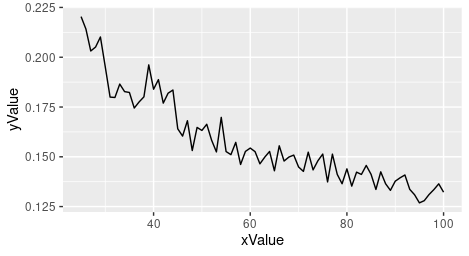
\includegraphics[width=10cm]{wykmse1.png} 

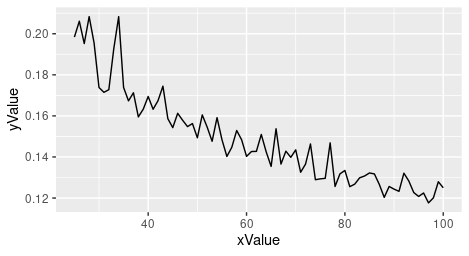
\includegraphics[width=10cm]{wykmse2.png}


\section*{Pełny program w R}
\begin{verbatim}
n <- 100
theta <- 1
omega <- 2
e3 <- function(X){ X[1] }
e4 <- function(X){
  X<- sort(X)
  ANS<-c()
  iter <- 0
  for(i in 1:length(X)){
    ANS <- append(ANS, (dnorm(qnorm(iter+0.0000001)) -dnorm(qnorm(iter+ 1/length(X)-0.0000001))))
    iter <- iter + 1/length(X)
  }
  return(sum(X*ANS))
}
mean_ans <- c()
median_ans <- c()
first_ans <- c()
weigh_ans <- c()
for(i in 1:10000){
  data <- rnorm(n,theta,omega)
  mean_ans <- append(mean_ans,mean(data))
  median_ans <- append(median_ans,median(data))
  first_ans <- append(first_ans,e3(data))
  weigh_ans <- append(weigh_ans,e4(data))
}
var_mean_ans <- var(mean_ans)
var_median_ans <- var(median_ans)
var_first_ans <- var(first_ans)
var_weigh_ans <- var(weigh_ans)

mse_mean_ans <- mean((mean_ans-theta)^2)
mse_median_ans <- mean((median_ans-theta)^2)
mse_first_ans <- mean((first_ans-theta)^2)
mse_weigh_ans <- mean((weigh_ans-theta)^2)

b_mean_ans <- mean(mean_ans)-theta
b_median_ans <- mean(median_ans)-theta
b_first_ans <- mean(first_ans)-theta
b_weigh_ans <- mean(weigh_ans)-theta

X <- c()
n<-50
newtons_method <- function(f,df,x,k){
  for(i in 1:k){
    x <- x-10^(-1)*(f(x)/df(x))
    #print(x)
  }
  if(is.na(x) || is.infinite(x)){
    return(NaN)
  }
  if(f(x) < 10^(-6)&&abs(x-0.7)<0.5){
    return (x)
  }else {
      return(NaN)
  }
}

location <- 1
scale <- 2
log_fun <- function(theta){ -sum(tanh((theta-X)/(2*scale))/scale)}
dlog_fun <- function(theta){ sum(-1/((scale^2*(cosh((theta*X)/scale)+1))))}
cau_fun <- function(theta){ sum((2*(X-theta)/(theta^2-2*theta*X+X^2+scale^2)))}
dcau_fun <- function(theta){ sum((2*(theta^2-2*theta*X+X^2-scale^2)
/(theta^2-2*theta*X+X^2+scale^2)^2))}
odp <- c()
i<-0
while(i < 10000){
  #X <- rlogis(n, location, scale)
  X <- rcauchy(n, location, scale)
  tmp <- newtons_method(cau_fun,dcau_fun,0.7,10^3)
  if(!is.na(tmp)){
    odp <- append(odp,tmp)
    i <- i+1
  }
  print(length(odp))
}
odp_var <- var(odp)
odp_mse <- mean((odp-location)^2)
odp_b <- mean(odp)-location


\end{verbatim}

\end{document}
